\chapter{Markov链与决策}\label{chap:markov-chain}

\begingroup
\newcommand{\pref}{Chapters/Markov-chain/figures}

\renewcommand{\P}{\mathcal P}
\newcommand{\MS}{\mathcal S}
\newcommand{\M}{\mathcal M}

\section{Markov链}

概率的解释

\begin{itemize}
    \item 回顾:我们在第一次课说过,似然,或者说合情推理的合理程度,是一种概率的解释模型.
    \item 尽管概率论在数学上通常被形式化为Kolmogorov公理体系,但是公理体系并没有回答``概率''是什么.
    \item 概率的解释是一个哲学课题. 两个主要的例子:
    \begin{itemize}
    \item 频率解释:概率是无穷次独立重复试验的频率(大数定律).
    \item 主观解释(Bayes解释):概率是对命题合理程度的信念(似然).
    \end{itemize}
\end{itemize}


{主观解释的缺陷}
\begin{itemize}
    \item 主观解释对推理的假设是逻辑的、静态的,时间的概念并不出现在似然里面.
    \item 例:考虑一个罐子,里面有除颜色之外不可区分的$N$个球,有$n$个白球,剩下的是黑球. 顺序从中拿出$N$个球,第$k$次拿出的球颜色是$W_k$或$B_k$.
    \begin{itemize}
        \item $\Pr(W_iW_j)=\Pr(W_i|W_j)\Pr(W_j)=\Pr(W_j|W_i)\Pr(W_i)$.($i<j$)
        \item $\Pr(W_i)=\Pr(W_j)=n/N\implies\Pr(W_i|W_j)=\Pr(W_j|W_i)$.
    \end{itemize}
    \item 从似然的角度,$\Pr(W_i|W_j)$和$\Pr(W_j|W_i)$不仅是可计算的,而且是相等的. 概率的计算告诉了我们,更早状态的信息依赖于未来的状态!
    \item 逻辑上蕴含关系并不意味着实际上的因果关系,但是似然完全没有考虑这一点. 因此,我们需要引入一个带有时间的模型,这就是Markov链.
\end{itemize}


{Markov链}
\begin{itemize}
    \item \emph{Markov链}(马氏链,Markov chain)是一个随机变量序列$\{X_t\}_{t=0}^{\infty}$. 包含如下概念:
\begin{itemize}
	\item 状态空间 $\MS$:$X_t$所有可能值构成的集合,有限或者可数.
	\item 转移矩阵 $\P$:下一时刻系统状态之间转移的概率.
		\begin{itemize}
        \item $\P=(p_{ij})_{i,j\in \MS}$,$p_{ij}$是从$i$状态转移到$j$状态的概率.
		\end{itemize}		
		\item \emph{Markov性}(Markov property): 对任意时刻$t=1,\dots,n$和任意状态$j,k,j_0,\dots,j_{t-1}\in \MS$,如下等式成立
		\begin{align*}
		   &\Pr(X_{t+1}=j| X_t=k,X_{t-1}=j_{t-1},\dots,X_0=j_0)\\
		   =& \Pr(X_{t+1}=j| X_{t}=k)=p_{kj}.
		\end{align*}
    \end{itemize}
	\item 注:我们给出的定义是简化的Markov链,每个时刻之间的转移都是一样的转移矩阵,这样的Markov链被称为\emph{时齐的}(time-homogeneous).
\end{itemize}


{Markov链}
\begin{itemize}
    \item Markov链是一种简化的带时间的概率模型.
    \item Markov性:在固定现在的情况下,过去与未来相互独立.
    \begin{itemize}
        \item 条件在$X_n=i$下,$\{Y_m\}_{m=0}^{\infty}:=\{X_{m+n}\}_{m=0}^{\infty}$是一个转移矩阵为$P$的Markov链,并且与$(X_0,\dots,X_{n-1})$相互独立. % HW: 证明这个命题
    \end{itemize}
    \item 时齐性:状态的转移不依赖当前时间,只和当前的状态有关.
    \begin{itemize}
        \item  $\Pr(X_{m+n}=j| X_{n}=k)=\Pr(X_{m}=j| X_{0}=k)$.
    \end{itemize}
    \item 有时候也会考虑带初态的Markov链,$X_0$服从分布$\lambda=(\lambda_s)_{s\in \MS}$.
\end{itemize}


{Markov链的例子}
\begin{itemize}
    \item 公平对赌. 玩家$A$和$B$抛硬币来赌钱,$A$赌正面,$B$赌反面.
    \item 每一轮独立地抛硬币,正面朝上的概率和反面朝上的概率相等,都是$1/2$. 赢的一方给输的一方一块钱. $A$输$a$块钱破产,$B$输$b$块钱破产,
    \item $Z_i$是第$i$轮$A$的收入. $Z_0=X_0=0$是$A$初始的收入. $X_n=Z_0+\dots+Z_n$是$A$的累计收入.
    \item 那么,$\{X_n\}_{n\geq 0}$是一个Markov链.
    \begin{itemize}
        \item 状态空间:$\MS=\{-a,-a+1,\dots,0,1,\dots,b\}$.
        \item 转移概率:对$-a<i<b-1$,$p_{i,i+1}=p_{i+1,i}=1/2$;$p_{-a+1,-a}=p_{b-1,b}=1/2$,$p_{-a,-a}=p_{b,b}=1$;其他值为$0$.
    \end{itemize}
\end{itemize}


{Markov链的例子}
\begin{itemize}
    \item  $\{X_n\}_{n\geq 0}$是一个Markov链.
    \begin{itemize}
        \item 状态空间:$\MS=\{-a,-a+1,\dots,0,1,\dots,b\}$.
        \item 转移概率:对$-a<i<b$,$p_{i,i+1}=p_{i+1,i}=1/2$;$p_{-a+1,-a}=p_{b-1,b}=1/2$,$p_{-a,-a}=p_{b,b}=1$;其他值为$0$.
    \end{itemize}
\end{itemize}
\begin{figure}[ht]
    \centering
    \includegraphics[width=0.8\textwidth]{\pref/gampling.eps}
\end{figure}


{赌徒谬误}
\begin{itemize}
    \item $A$的累计收入$\{X_n\}_{n\geq 0}$形成了Markov链.
    \item 根据Markov性,未来双方的收入变化只取决于现在,而和过去运气无关.
    \item 赌徒谬误(gambler's fallacy):深陷赌局中的人会按照自己历史上的运气来评估自己未来的运气,认为过去运气差未来运气就会变好.
    \item ``风水轮流转''在一场公平对赌中是不正确的认知.
    \item 思考:如何评估赌局的公平性?
\end{itemize}


{多步转移概率}
\begin{itemize}
    \item 如果对赌是公平的,那么我们应该认为两个人每一轮的累计收入分布都是一样的,即
    \[\Pr(X_n=i|X_0=0)=\Pr(X_n=-i|X_0=0).\]
    \item 因此,我们需要能够计算多步转移的概率.
    \item 设$p_{ij}^{(k)}$表示从状态$i$用$k$步转移到状态$j$的概率.
    \item $k$步转移概率形成了一个矩阵$\P^{(k)}$.
    \item Kolmogorov-Chapman方程:
    \[\P^{(k+l)}=\P^{(k)}\P^{(l)}.\]
\end{itemize}



{多步转移概率}
\begin{itemize}
    \item Kolmogorov-Chapman方程:
    \[\P^{(k+l)}=\P^{(k)}\P^{(l)}.\]
    \item 证明:由Markov性、时齐性和全概率公式,$
        p_{ij}^{(k+l)}=\Pr(X_{k+l}=j|X_0=i)=\sum_{\alpha}\Pr(X_{k+l}=j,X_k=\alpha|X_0=i)=\sum_{\alpha}\Pr(X_k=\alpha|X_0=i)\Pr(X_{k+l}=j|X_k=\alpha)=\sum_{\alpha} p_{i\alpha}^{(k)}p_{\alpha j}^{(l)}$.
    \item 特例:前向方程(forward equation)$\P^{(k+1)}=\P^{(k)}\P$,后向方程(backward equation)$\P^{(l+1)}=\P\P^{(l)}$.
    \item 推论:$\P^{(k)}=\P^k$.
    \item 若已知初始分布向量为$\lambda$,我们可以计算它随时间的演化:
		\[\lambda^\t,\lambda^\t \P,\dots,\lambda^\t \P^n,\dots\] %HW: 证明这个演化
\end{itemize}


{多步转移概率}
\centering
\begin{minipage}[t]{0.4\textwidth}
前向方程(往前一步):
    \centering
    \includegraphics[width=0.6\textwidth]{\pref/forward-equation.eps}
\end{minipage}
\begin{minipage}[t]{0.4\textwidth}
后向方程(往回一步):
    \centering
    \includegraphics[width=0.6\textwidth]{\pref/backward-equation.eps}
\end{minipage}


{遍历定理与平稳分布}
\begin{itemize}
	\item 思考:如何计算公平对赌中$X_n$的概率分布?
	\item 我们先来看一个简单的例子. 假设$|p_{00}+p_{11}-1|<1$,考虑只有两个状态$0,1$,转移矩阵为
	\[\P=\begin{pmatrix}p_{00}&p_{01}\\p_{10}&p_{11}
	\end{pmatrix}.\]
\end{itemize}
\begin{figure}
    \centering
    \includegraphics[width=0.4\textwidth]{\pref/simple-example.eps}
\end{figure}


{遍历定理}
\begin{itemize}
	\item 可以归纳证明:
	\begin{align*}
	    \P^n=&\frac{1}{2-p_{00}-p_{11}}\begin{pmatrix}1-p_{11}&1-p_{00}\\1-p_{11}&1-p_{00}\end{pmatrix}\\
	    &+\frac{(p_{00}+p_{11}-1)^n}{2-p_{00}-p_{11}}\begin{pmatrix}1-p_{00}&-(1-p_{00})\\-(1-p_{11})&1-p_{11}\end{pmatrix}.
	\end{align*}
	\item $\lim_{n\to\infty}p_{i0}^{(n)}=(1-p_{11})/(2-p_{00}-p_{11})$,$\lim_{n\to\infty}p_{i1}^{(n)}=(1-p_{00})/(2-p_{00}-p_{11})$.
	\item 随着时间的推移,Markov链初始状态对概率分布的影响逐渐消失. 这个规律具有普遍性,这就是遍历定理.
\end{itemize}


{遍历定理}
\begin{theorem}[遍历定理,Ergodic theorem]
Markov链的状态空间为$\MS=\{1,\dots,N\}$,转移矩阵为$\P=(p_{ij})$.
\begin{itemize}
    \item 如果对于某一个$n_0$有
    \begin{equation}
        \min_{ij}p_{ij}^{(n_0)}>0,\label{eq:reachable}
    \end{equation}
    那么存在分布$\lambda=(\lambda_1,\dots,\lambda_N)$使得
    \begin{equation}
        \lambda_i>0,\quad\sum_i\lambda_i=1,\label{eq:positive-distribution}
    \end{equation}
    并且对于每一个$j\in\MS$和任意$i\in\MS$都有
    \begin{equation}
    p_{ij}^{(n)}\to\lambda_j,n\to\infty.\label{eq:converge-to-limit}
    \end{equation}
\end{itemize}
\end{theorem}


{遍历定理}
\begin{theorem}[遍历定理,续]
\begin{itemize}
    \item 反之,如果存在满足 \eqref{eq:positive-distribution} 和 \eqref{eq:converge-to-limit} 的$\lambda$,则存在满足 \eqref{eq:reachable} 的$n_0$.
    \item 式 \eqref{eq:positive-distribution} 的$\lambda$满足
    \begin{equation}
        \lambda^\t = \lambda^\t\P.\label{eq:stationary}
    \end{equation}
\end{itemize}
\end{theorem}
\begin{itemize}
    \item 条件 \eqref{eq:reachable} 表明超过某个步数$n_0$之后,从$i$出发到达$j$的概率总是正的,这个条件被称为\emph{遍历}(ergodic).
    \item 条件 \eqref{eq:positive-distribution} 表明每一个状态被访问到的概率都是正的,没有``死状态''.
    \item 遍历定理表明遍历的Markov链从任何状态出发都是不可逆的,最终会把每个状态都走过一遍(遍历),变成一个混合均匀的状态.
    \begin{itemize}
        \item 这可以用来解释物理学中的扩散现象. % HW: 算一下Ehrenfest模型
    \end{itemize}
\end{itemize}


{平稳分布}
\begin{itemize}
    \item 满足条件 \eqref{eq:stationary} 的分布被称为\emph{平稳分布}(stationary distribution).
    \item 平稳分布为初始状态时,Markov链的演化与时间无关:$(X_k,\dots,X_{k+l})$的联合分布不依赖于$k$.
    \item 如果Markov链是遍历的,那么平稳分布是唯一的.
    \begin{itemize}
        \item 假设$\mu$是另外一个平稳分布,那么$\mu_j=\sum_\alpha\mu_\alpha p_{\alpha j}=\dots=\sum_{\alpha}\mu_\alpha p_{\alpha j}^{(n)}$.
        \item 因为$p_{\alpha j}^{(n)}\to \lambda_j$,所以$\mu_j=\sum_{\alpha} (\mu_\alpha\lambda_j)=\lambda_j$.
    \end{itemize}
    \item 非遍历Markov链也可能存在(唯一)平稳分布,考虑$\P=\begin{pmatrix}0&1\\1&0\end{pmatrix}$和$\lambda=(1/2,1/2)^\t$.
\end{itemize}


\section{Markov奖励过程(MRP)}
{决策理论}
\begin{itemize}
    \item 我们接下来的目标就是在Markov链上建立决策理论.
    \item 每一阶段我们可以选择某个行动,这个行动在Markov链会产生一些奖励.
    \item 我们的目标是选择恰当的行动方式是的我们的总奖励最大.
    \item 首先我们定义奖励的过程.
\end{itemize}

{Markov奖励过程}
\begin{itemize}
\item 一个\emph{Markov奖励过程}(Markov reward process,MRP)是四元组$\langle\MS,\P,\mathcal R,\gamma\rangle$:
\begin{itemize}
    \item $\MS$是一个有穷的状态集合.
    \item $\P$是一个状态转移矩阵,从$i$转移到$j$的概率记为$\P_{i,j}$.
    \item $\mathcal R$是一个奖励函数,$\mathcal R_s = \E[\textcolor{red}{R_{t+1}}|S_t=s]$:当$t$时刻位于状态$s$时 下一时刻(离开)获得的奖励的期望,$\textcolor{red}{R_{t+1}}$是下一阶段所处状态的奖励.
    \item $\gamma$是一个折扣系数,$\gamma\in[0,1]$.
\end{itemize}
    \item 注:条件数学期望$\E[\cdot|S_t=s]$可以理解为条件在$\{S_t=s\}$下定义的概率所求的期望.
\end{itemize}


{例子:学生MRP}
\begin{figure}
    \centering
    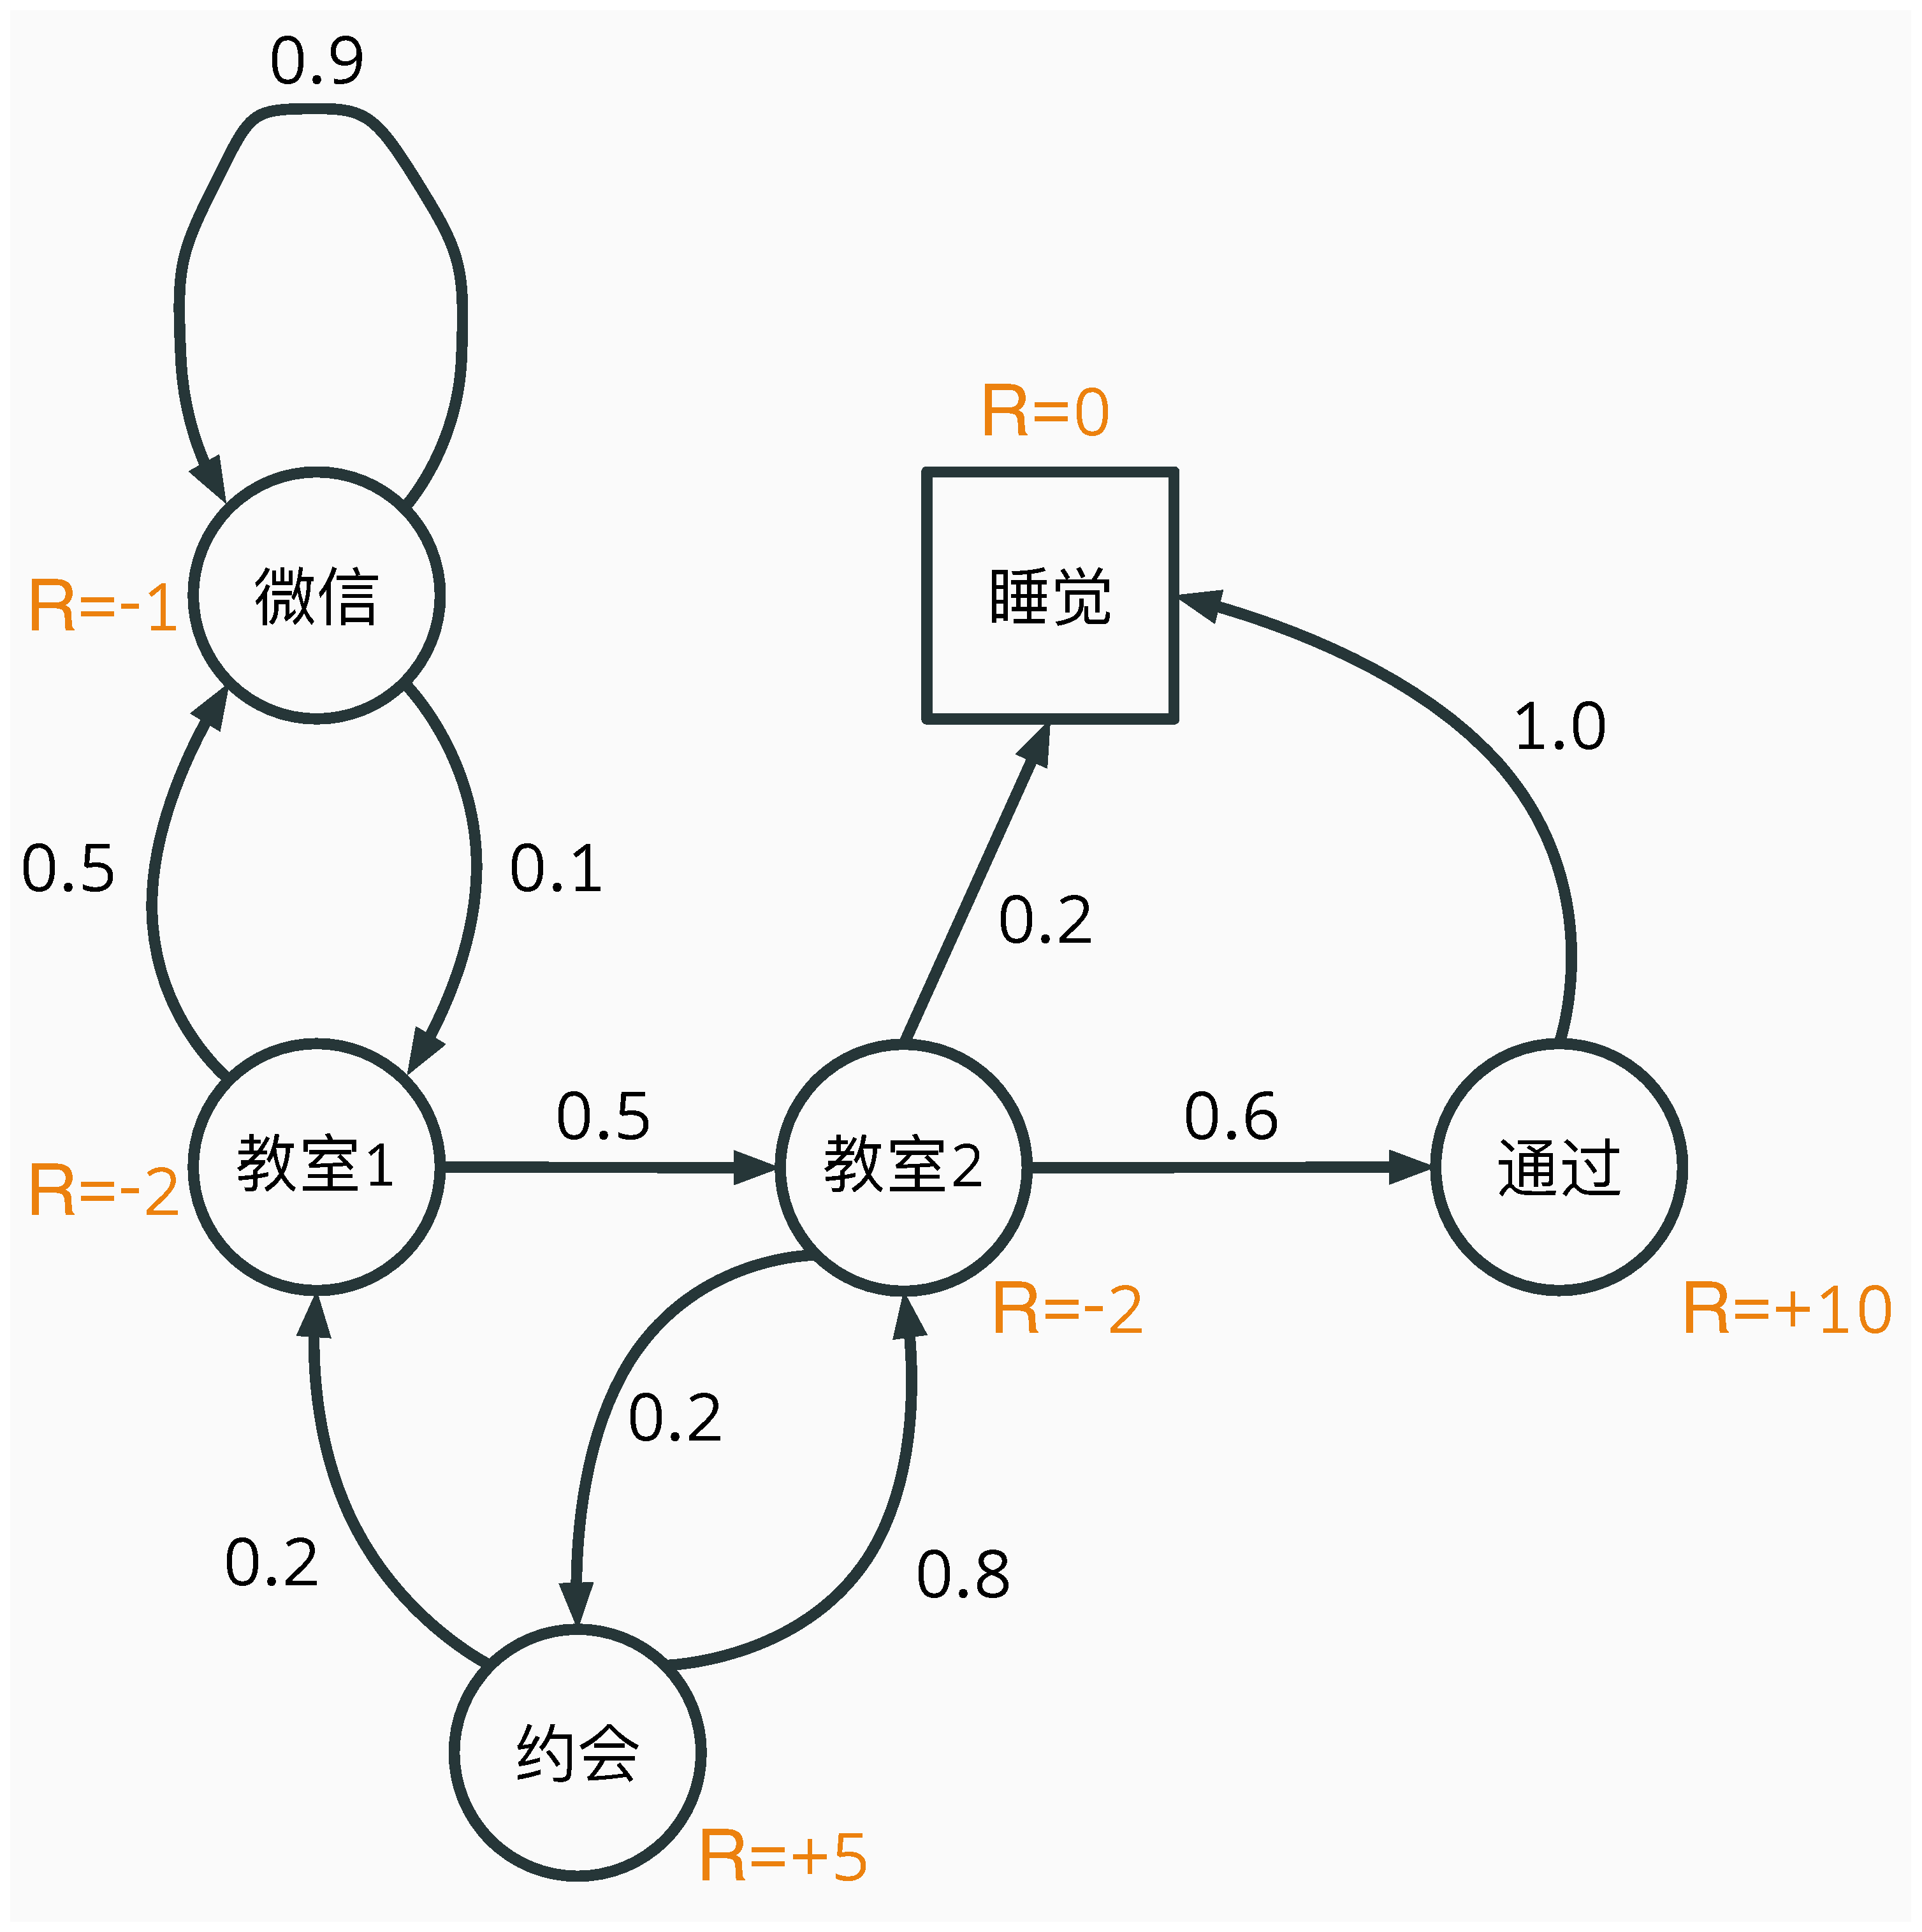
\includegraphics[height=0.8\textheight]{\pref/STR.eps}
\end{figure}


{回报}
\begin{itemize}
    \item MRP中,$t$时刻以后的总\emph{回报}(Return)$G_t$定义为
    \[G_t = R_{t+1}+\gamma R_{t+2} +\dots =\sum_{k=0}^\infty \gamma^kR_{t+k+1}.\]
        \item $\gamma \in[0,1]$衡量了未来下一时段1的奖励在当前时刻的价值.
        \item 未来$k+1$时刻的奖励对当前时刻$t$的作用是$\gamma^k R_{t+k+1}$.
        \item 若$\gamma\to0$,表示对奖励进行“短视”的评估;反之更“远见”.
\end{itemize}


{折扣系数的意义}
\begin{itemize}
    \item 许多MRP和后面学习的MDP都有与时间无关的折扣系数$\gamma <1$,原因:
\begin{itemize}
    \item 起始于对未来不确定性对冲:直接对应于利润率. 
    %具有不确定性,因此未来的回报更有风险,需要一个折扣风险的系数.
    %\item 数学上表示不麻烦.
    \item 动物和人类对即时回报具有偏好.
\end{itemize}
\item 有时也使用非折扣化的MRP(即$\gamma=1$),例如当所有的转移序列都会有固定的终止时间.
\end{itemize}


{价值函数}
\begin{itemize}
    \item 在MRP中,状态\emph{价值函数}(value function)$v(s)$表示从状态$s$出发的期望回报
    \[v(s) = \E(G_t|S_t=s).\]
    \item 价值函数$v(s)$衡量了状态$s$的长期效益.
    \item Markov性:只从当前起考虑未来收益,不考虑历史收益(沉没成本)的影响.
    \item 时齐性:价值函数的定义不依赖于时刻$t$
    (无穷阶段情形).
\end{itemize}



{MRP的Bellman方程}
\begin{itemize}
    \item 价值函数可以被分解为两部分:
\begin{itemize}
    \item 即时回报$\textcolor{red}{R_{t+1}}$
    \item 下一个状态开始的折扣价值 $\textcolor{green}{\gamma v(S_{t+1})}$
\end{itemize}
        \begin{align*}
        v(s) &= \E(G_t|S_t=s) \\
            &= \E(R_{t+1}+ \gamma R_{t+2} + \gamma^2 R_{t+3}+\dots | S_t= s) \\
            &= \E(R_{t+1} + \gamma (R_{t+2}+\gamma R_{t+3}+\dots) | S_t = s) \\
            &= \E(R_{t+1} + \gamma G_{t+1} | S_t = s) \\
            &= \E(\textcolor{red}{R_{t+1}} + \textcolor{green}{\gamma v(S_{t+1})}| S_t=s)\\
            &= {\textcolor{red}{\mathcal R_s} + \textcolor{green}{\gamma \sum_{s'\in \MS}\P_{s,s'}v(s')}}. % HW: 做一下破产博弈的Wald等式. 看一下zfx应随教材1.10三(100页),可以在题目里直接假设停时概率1有限
    \end{align*}
\end{itemize}


{矩阵形式的Bellman方程}
\begin{itemize}
    \item Bellman方程可以用矩阵形式表达:
        \[v = \mathcal R + \gamma \mathcal P v.\]
    这里$v$是列向量$v=(v(s))_{s\in\MS}$.
\end{itemize}


{Bellman方程的解}
\begin{itemize}
    \item Bellman方程是一个线性方程,可以被直接解:
    \[
        v =\mathcal R + \gamma \P v \implies (I-\gamma \P)v = \mathcal R \implies v = (I-\gamma \P)^{-1} \mathcal R.
   \]
    \item 对于$n$个状态的Markov链,计算复杂度为$\O(n^3)$.
    \item 对于较小的MRP可以直接解,太大的MRP开销太大.
    \item 对于大型MRP,可以采用迭代算法,例如:
    \begin{itemize}
        \item 动态规划(dynamic programming)
        \item Monte-Carlo评估(Monte-Carlo evaluation) 
        \item 时序差分学习(temporal-difference learning)
    \end{itemize}
\end{itemize}


\section{Markov决策过程(MDP)}
{Markov决策过程}
\begin{itemize}
    \item \emph{Markov决策过程}(Markov decision process)是一个定义了决策的MRP. 它可以看做一个任意状态都具有Markov性的\emph{环境}.
    \item 一个MDP是五元组$\langle\MS, \textcolor{green}{\mathcal A}, \P, \mathcal R, \gamma\rangle$.
        \begin{itemize}
            \item $\MS$是一个有限的状态集合.
            \item $\textcolor{green}{\mathcal A}$是一个有限的\emph{行动}(action)集合.
            \item $\P$是状态转移概率矩阵,
            \[\P_{ss'}^{\textcolor{green}{a}} = \Pr(S_{t+1} = s' | S_t = s, A_t = \textcolor{green}{a}).\]
            \item $\mathcal R$是一个奖励函数,$\mathcal R_s^{\textcolor{green}{a}} = \E(\textcolor{red}{R_{t+1}} | S_t = s, A_t = \textcolor{green}{a})$,$\textcolor{red}{R_{t+1}}$是进行某一行动到达某一状态后的奖励.
            \item $\gamma$是一个折扣系数$\gamma\in[0,1]$.
        \end{itemize}
    \end{itemize}


{例子:学生MDP}
\begin{figure}
    \centering
    \includegraphics[height=0.8\textheight]{\pref/STD.eps}
\end{figure}


{策略}
\begin{itemize}
    \item     一个\emph{策略}(policy)$\pi$是给定状态下行动的分布,
    \[\pi(a|s) = \Pr(A_t=a | S_t = s).\]
    \item 一个策略完全决定了一个智能体在MDP环境中的行为.
    \item Markov性:MDP的策略取决于当前状态,而非历史状态.
    \item 时齐性:MDP的策略不依赖于时刻$t$.
\end{itemize}


{策略}
\begin{itemize}
    \item 给定一个MDP $\M=\langle\MS,\mathcal A,\P,\mathcal R, \gamma\rangle$和一个策略$\pi$.
    \item $\langle \MS, \P^{\pi}\rangle$是一个Markov链.
    \item $\langle\MS,\P^{\pi}, \mathcal R^{\pi}, \gamma\rangle$是一个MRP.
    \item 其中
\end{itemize}
\[\P_{s,s'}^{\pi} = \E_{a\sim\pi(\cdot|s)}(\P^a_{s,s'})=\sum_{a\in \mathcal A}\pi(a|s)\mathcal P_{s,s'}^{a},\]
    \[\mathcal R_s^{\pi} =\E_{a\sim\pi(\cdot|s)}(\mathcal R^a_s)=\sum_{a\in\mathcal A}\pi(a|s)\mathcal R_s^a.\]


{价值函数}
\begin{itemize}
    \item 在MDP中,状态-价值函数$v_\pi(s)$是从状态$s$出发,遵从策略$\pi$的期望回报
    \[v_\pi(s) = \E_\pi(G_t|S_t=s).\]
    \item     行动-价值函数$q_\pi(s,a)$是从状态$s$出发,采取行动$a$,遵从策略$\pi$的期望回报
    \[q_\pi(s,a) = \E_\pi(G_t|S_t=s,A_t=a).\]
    \item 注意,以上定义都具有Markov性和时齐性.
\end{itemize}


{Bellman期望方程}
\begin{itemize}
    \item 状态-价值函数可以被分解为:即时回报 加 后续状态的折扣价值,
\[v_\pi(s) = \E_\pi(R_{t+1} + \gamma v_\pi(S_{t+1})|S_t=s).\]
\item 行动-价值函数可以被类似地分解,
\[q_\pi(s,a) = \E_\pi(R_{t+1} + \gamma q_\pi(S_{t+1},A_{t+1})|S_t=s,A_t=a).\]
\item 二者之间的关系(全概率公式、一步转移概率):
\[q_\pi(s,a) =\mathcal R_s^a + \gamma \sum_{s'\in \MS}P_{s,s'}^a v_\pi(s').\]
\[v_\pi(s) = \E_{a\sim\pi(\cdot|s)}(q_\pi(s,a))=\sum_{a\in\mathcal A}\pi(a|s)q_\pi(s,a),\]
\end{itemize}


{Bellman期望方程}
\begin{itemize}
    \item 因此,我们得到MDP的Bellman期望方程:
\[v_\pi(s) = \sum_{a\in \mathcal A}\pi(a|s)\left(\mathcal R_s^a + \gamma \sum_{s'\in \MS}\P_{s,s'}^av_\pi(s')\right),\]
\[q_\pi(s,a) = \mathcal R_s^a + \gamma \sum_{s'\in \MS}\P_{s,s'}^a \sum_{a'\in \mathcal A}\pi(a'|s')q_\pi(s',a').\]
\item 矩阵形式:
\[v_\pi = \mathcal R^\pi + \gamma \P^\pi v_\pi = (I-\gamma \mathcal P^\pi)^{-1}\mathcal R^\pi.\]
\end{itemize}


{最优价值函数}
\begin{itemize}
    \item \emph{最优状态-价值函数} $v_\star(s)$ 是所有决策中最大的状态-价值函数
    \[v_\star(s) = \max_\pi v_\pi(s).\]
    \item \emph{最优行动-价值函数} $q_\star(s,a)$是所有决策中最大的行动-价值函数
    \[q_\star(s,a) = \max_\pi q_\pi(s,a).\]
    \item 最优价值函数确定了MDP中的最佳收益.
    \item 解MDP即确定达到最优价值函数的策略.
\end{itemize}


{最优策略}
\begin{itemize}
    \item 然而,每个状态取到最大价值的策略$\pi$可能并不是同一个.
    \item 幸运的是,确实存在一个这样的最优策略. 定义一个策略的偏序:
    \[\pi\ge\pi' \iff \forall s\in\MS\ v_\pi(s) \ge v_{\pi'}(s).\]
\end{itemize}
\begin{theorem}[MDP解的存在性]
对任意MDP,
\begin{itemize}
    \item 存在一个最优策略 $\pi_\star$使得$\forall \pi\ \pi_\star\ge\pi$.
    \item 最优策略取得最优状态-价值函数:$v_{\pi_\star}(s) = v_\star(s)$.
    \item 最优策略取得最优行动-价值函数:$q_{\pi_\star}(s,a)=q_\star(s,a)$.
\end{itemize}
\end{theorem}


{寻找最优决策}
\begin{itemize}
    \item 可以通过最大化$q_\star(s,a)$来寻找:
    \begin{itemize}
        \item 固定$s$.
        \item 找到一个$a_\star$使得$q_\star(s,a_\star)=\max_{a}q_\star(s,a)$,令$\pi_\star(a_\star|s)=1$.
        \item 对$\forall a\neq a_\star$,$\pi_\star(a|s)=0$.
    \end{itemize}
    \item 证明:根据选法,$\pi_\star$取得最优行动-价值函数.
    \item 由$v_\pi(s) = \E_{a\sim\pi(\cdot|s)}(q_\pi(s,a))\leq \E_{a\sim\pi(\cdot|s)}(q_\star(s,a))\leq q_\star(s,a_\star)=v_{\pi_\star}(s)$知$\pi_\star$取得最优状态-价值函数.
    \item 推论:对任意MDP,总存在一个非随机的最优决策.
    \item 如果我们知道$q_\star(s,a)$,我们就能获得最优决策. % HW: 找一个简单一点的例子,让他们算一下最优策略
\end{itemize}


{Bellman最优性方程}
\begin{itemize}
    \item 最优价值函数由Bellman最优性方程联系:
\[v_\star(s) = \max_a q_\star(s,a),\]
\[q_\star(s,a) = \mathcal R_s^a + \gamma \sum_{s'\in \MS}\P_{s,s'}^av_\star(s'),\]
\[v_\star(s) = \max_a\left\{\mathcal R_s^a + \gamma \sum_{s'\in \MS}\P_{s,s'}^av_\star(s')\right\},\]
\[q_\star(s,a) = \mathcal R_s^a+\gamma \sum_{s'\in \MS}\P_{s,s'}^a\max_{a'}q_\star(s',a').\]
\end{itemize}


{解Bellman最优性方程}
    \begin{itemize}
        \item Bellman最优性方程不是线性的. 因此没有解析形式的(closed form)解.
        \item 但是MDP的数值解是可以多项式时间求出来的.
        \item 我们一般采用迭代算法求解:
        \begin{itemize}
            \item 价值迭代(value iteration)
            \item 策略迭代(policy iteration)
            \item Q-learning
            \item Sarsa
        \end{itemize}
    \end{itemize}

{关于Bellman方程}
\begin{itemize}
    \item Bellman方程是强化学习(reinforcement learning)、经济学动态优化(dynamic optimization)的核心.
    \item Bellman方程的推导是Markov链中最为常用的技巧:考虑从当前状态转移到下一状态,利用全概率公式,一步转移会将两个状态之间的概率(期望)用递推公式联系起来.
    \begin{itemize}
        \item 随机过程中的例子:前向方程、Wald等式、调和函数(harmonic function).
        \item 后面的HMM也是类似的例子.
    \end{itemize}
\end{itemize}


\section{隐Markov模型(HMM)}

问题的引入

\begin{itemize}
    \item 我们考虑Markov链上的另一种应用.
    \item 在统计学和机器学习中,我们有时候要处理一类含时间的数据.
    \item 最简单的情况是回归,即数据完全由所处时刻决定.
    \item 但是通常,现在的数据依赖于过去的数据.
    \item 因此,一种最简单的考虑就是数据依赖于Markov链,这就是隐Markov模型.
\end{itemize}


{隐Markov模型}
\begin{itemize}
    \item 一个\emph{隐Markov模型}(hidden Markov model,HMM)是一列随机变量$X_1,X_2,\dots, X_t$,满足:
    \begin{itemize}
        \item $X_t$的分布仅依赖于隐状态$Z_t$,即$\Pr(X_1,\dots,X_t|Z_1,Z_2,\dots,Z_t)=\prod_i \Pr(X_i|Z_i)$.
        \item $\{Z_t\}$构成一条Markov链.
    \end{itemize}
\end{itemize}
\begin{figure}
    \centering
    \includegraphics[width=0.6\textwidth]{\pref/HMM.eps}
\end{figure}


{有限观测HMM}
\begin{itemize}
    \item 一个HMM包含:
    \begin{itemize}
        \item $\mathcal Z$
        : 有限的状态集合.
        \item $\mathcal X$: 有限的观测集合.
        \item $T: \mathcal Z\times\mathcal Z\to \R_{\geq 0}$,$\mathcal Z$的转移概率.
        \item $M:\mathcal Z\times \mathcal X\to \R_{\geq 0}$,给定状态时的观测概率(条件概率).
        \item $\lambda:\mathcal Z\to\R_{\geq 0}$,初始状态的先验概率分布列.
    \end{itemize}
    \item 如果随机过程$\{X_t\}$的值域是有限集,我们则可以用矩阵表达HMM.
    \begin{itemize}
    \item $T$是$\{Z_t\}$的转移矩阵.
    \item $M$是观测矩阵:$M_{i,k} = \Pr(X_t=k|Z_t=i)$.
    \item $\lambda$是一个概率向量.
    \end{itemize}
\end{itemize}


\subsection{评估问题}
{HMM的评估}
\begin{itemize}
   \item 给定一个特定的HMM,它对实际观测序列的拟合程度有多好?
   \item 记号:随机向量$X=(X_1,\dots,X_t)$,$Z=(Z_1,\dots,Z_t)$.
   \item  HMM的\emph{评估}(evaluation)问题:给定一个HMM $\M$,以及它的观测历史$x=(x_1,x_2,\dots,x_t)$,计算$\Pr(X=x|\M)$.
   \item 关键困难:我们不知道状态历史$Z=(z_1,z_2,\dots,z_t)$.
\end{itemize}


{朴素方法}
    \begin{itemize}
    \item 直接使用条件概 率进行推导:
    \[
        \Pr(X=x|\M) =\sum_{Z=(z_1, \dots, z_t) \in \mathcal Z} \Pr(X=x|Z=z, \M)\Pr(Z=z|\M),
    \]
    \[
        \Pr(X=x|Z=z,\M) = \prod_{i=1}^t \Pr(X_i = x_i| Z_i = z_i) = M_{z_1,x_1}\cdot M_{z_2,x_2}\dots M_{z_t,x_t},
    \]
    \begin{align*}
        \Pr(Z=z|\M) &= \Pr(Z_1 = z_1) \prod_{i=2}^t\Pr(Z_i = z_i| Z_{i-1} = z_{i-1}) 
        \\
        &= \lambda_{z_1}\cdot T_{z_1,z_2}\cdot T_{z_2,z_3}\dots T_{z_{t-1},z_t}.
    \end{align*}
    \item 时间复杂度: $\O(t|\mathcal Z|^t)$.
    \end{itemize}


{前向算法}
    \begin{itemize}
    \item 思路:类似前向方程,我们可以从前$k$步的结果推出前$k+1$步的结果. 因此可以列出递推方程.
    \item 记号:$X_{i:j}=(X_i,\dots,X_j)$.
    \item 具体地,定义$\alpha_k(z):= \Pr(X_{1:k}=x_{1:k}, Z_k=z| \M)$,我们有
    \begin{itemize}
        \item $\alpha_1(z) = \lambda(z)M_{z,x_1}$.
        \item $\alpha_{k+1}(z) = \sum_{z' \in \mathcal Z}\alpha_{k}(z')T_{z',z}M_{z,x_{k+1}}$.
    \end{itemize}
    \item $\Pr(X=x| \M) = \sum_{z\in \mathcal Z}\alpha_t(z)$.
    \item 时间复杂度 $\mathcal O(t|\mathcal Z|^2)$.
\end{itemize}



{后向算法}
   \begin{itemize}
    \item 类似后向方程,从前$k+1$步的结果推出前$k$步的结果. 同样可以列出递推方程.
    \item 定义$\beta_k(z):=\Pr(X_{k+1:t}=x_{k+1:t} | Z_k=z,\M)$,我们有
    \begin{itemize}
        \item 当$k = t$,$\beta_k(z) = 1$.
        \item 当$1 \le k < t$,$\beta_{k}(z) = \sum_{z' \in \mathcal Z}T_{z,z'}M_{z',x_{k+1}}\beta_{k+1}(z')$.
    \end{itemize}
    \item $\Pr(X=x| \M) = \sum_{z\in \mathcal Z}\lambda(z)M_{z,x_1}\beta_1(z)$.
    \item 时间复杂度 $O(t|\mathcal Z|^2)$.
\end{itemize}


\subsection{解释问题}
{HMM的解释问题}
    \begin{itemize}
    \item HMM的\emph{解释}(explanation)问题:给定一个 HMM $\M = (\mathcal Z, \mathcal X, T, M, \lambda)$, 一列观测历史$x = (x_1, x_2, \dots, x_t)$, 寻找一个状态序列,能最好地解释这些历史观察.
    \item 具体地,我们考虑如下四个问题
    \begin{enumerate}
        \item 过滤(filtering):计算$\Pr(Z_k = s|X_{1:k}=x_{1:k}, \M)$.
        \item 平滑(smoothing): 计算$\Pr(Z_k = s|X=x, \M)$,$k < t$.
        \item 预测(prediction): 计算$\Pr(Z_k = s|X=x, \M)$,$k > t$.
        \item 解码(decoding): 找到最有可能的状态序列 $z = (z_1, z_2, \dots, z_t)$.
    \end{enumerate}
\end{itemize}




{过滤:$\Pr(Z_k = s|X_{1:k}=x_{1:k}, \M)$}
\begin{itemize}
    \item 回顾:$\alpha_k(s)= \Pr(X_{1:k}=x_{1:k}, Z_k=s| \M)$. 
    \item 我们有
    \begin{align*}
        \Pr(Z_k = s|X_{1:k}=x_{1:k}, \M) & = \frac{\Pr(X_{1:k}=x_{1:k}, Z_k=s| \M)}{\Pr(X_{1:k}=x_{1:k}| \M)} \\
        &= \frac{\alpha_k(s)}{\sum_{z\in\mathcal Z}\alpha_k(z)}.
    \end{align*}
\end{itemize}


{平滑:$\Pr(Z_k = s|X=x, \M)$,$k < t$} 
\begin{itemize}
    \item 回顾:$\alpha_k(s)= \Pr(X_{1:k}=x_{1:k}, Z_k=s| \M)$.
    \item 回顾:$\beta_k(s)=\Pr(X_{k+1:t}=x_{k+1:t} |Z_k=s, \M)$.
    \item 可以证明:
        \[\Pr(z_k = s|X=x, \M)=\frac{\beta_k(s)\alpha_k(s)}{\sum_{z\in\mathcal Z}\alpha_t(z)}.
    \]% HW: 推导这个
    % \[\Pr(X_k = s|z, \M) =& \frac{\Pr(z_{1:k}, z_{k+1:t}, X_k=s| \M)}{\Pr(z| \M)} 
    %     \\
    %     =& \frac{\Pr(z_{k+1:t}| z_{1:k}, X_k=s,\M)\Pr(z_{1:k}, X_k=s| \M)}{\Pr(z| \M)}
    %     \\
    %     =& \frac{\Pr(z_{k+1:t}| X_k=s,\M)\Pr(z_{1:k}, X_k=s| \M)}{\Pr(z| \M)}
    %     \\
    %     =& \frac{\beta_k(s)\alpha_k(s)}{\Pr(z| \M)} = \frac{\beta_k(s)\alpha_k(s)}{\sum_{x\in\mathcal X}\alpha_t(x)} 
    % \]
\end{itemize}



{预测:$\Pr(Z_k = s|X=x, \M)$,$k > t$.}
\begin{itemize}
    \item 首先用过滤计算 $\lambda=\Pr(Z_t = s|X=x, \M)$.
    \item 然后用 $\lambda$ 作为Markov的初始状态,向前计算$k-t$步.
\end{itemize}


{*解码:Viterbi算法}
\begin{itemize}
    \item 定义 
    $$\delta_k(s) = \max_{Z_{1:k-1}}\Pr(Z_{1:k} = (z_{1:k-1}, s), X_{1:k}=x_{1:k}| \M).$$
    \item 根据一步转移,我们有
    $$\delta_{k+1}(s) = \max_{q\in \mathcal Z}\{\delta_k(q)T_{q,s}\}M_{s,x_{k+1}}.$$
    \item 问题转化为: 记录最高概率的路径,这是一个动态规划问题.
\end{itemize}


\newcommand{\pre}{\mathrm{Pre}}
{*解码: Viterbi算法}
\begin{itemize}
    \item 初始化:
    \begin{itemize}
        \item $\delta_1(s) = \lambda(s)M_{s,z_1}$.
        \item $\pre_1(s) = \varnothing$.
    \end{itemize}
    \item 对 $k=1, 2, \dots, t-1$,$s \in \mathcal Z$:
    \begin{itemize}
        \item $\delta_{k+1}(s) = \max_{q\in \mathcal Z}\{\delta_k(q)T_{q,s}\}M_{s,x_{k+1}}$.
        \item $\pre_{k+1}(s) = \argmax_{q\in \mathcal Z}\{\delta_k(q)T_{q,s}\}$.
    \end{itemize}
    \item $z_t = \argmax_{s \in \mathcal Z}\delta_{t}(s)$.
    \item 对 $1 \le k < t$,$z_k = \pre_{k+1}(z_{k+1})$.
    \item 时间复杂度: $\mathcal O(t|\mathcal Z|^2)$.
\end{itemize}

\endgroup